\documentclass{article}
% Packages for language and encoding
\usepackage[utf8]{inputenc}
\usepackage[T1]{fontenc}
\usepackage[english]{babel}

% Packages for images and hyperlinks
\usepackage{graphicx}
\usepackage{hyperref}

% Package for verbatim environment
\usepackage{verbatim}

% Package for floating figures
\usepackage{float}

% Package for page geometry
\usepackage{geometry}
\geometry{a4paper, margin=1in}

\usepackage{tabularx}
\usepackage{caption}

\captionsetup[table]{font={small},skip=0pt, singlelinecheck=false, justification=raggedright}
\captionsetup[figure]{font={small},skip=0pt, singlelinecheck=false, justification=raggedright}

% Set up hyperref package
\hypersetup{
    colorlinks=true,
    linkcolor=blue,
    filecolor=magenta,
    urlcolor=cyan,
}

% Package for customizing title page
\usepackage{titling}
\usepackage{amsmath}

% Package for listings
\usepackage{listings}

% Document metadata
\title{Malicious IP-Address Monitor: Enhancing Internet Security}
\author{Pelletier Max \and Pernjak Stefani \and Rezzonico Marco \\ Advisor: Dr. Simon Kramer}
\date{\today}

% Customization for title page
\pretitle{\begin{center}\LARGE}
\posttitle{\par\end{center}\vskip 0.5em}
\preauthor{\begin{center}\large}
\postauthor{\par\end{center}\vskip 0.5em}
\predate{\begin{center}\large}
\postdate{\par\end{center}\vskip 0.5em}

\begin{document}

% Title Page
    \begin{titlepage}
        \vspace{0.1cm}
        \centering
        {\LARGE\bfseries Malicious IP-Address Monitor: Enhancing Internet Security \par}
        \vspace{1cm}
        {\Large Pelletier Max, Pernjak Stefani, Rezzonico Marco \par}
        \vspace{0.5cm}
        {\large Project 1 (BTI3031)\par}
        \vspace{0.5cm}
        {\large Advisor: Dr. Simon Kramer\par}
        \vspace{0.5cm}
        {\large Bern University of Applied Sciences\\Department of Computer Science\par}
        \vspace{0.5cm}
        {\Large Date: \today\par}
        \vspace{3cm}
        \centering
        
\includegraphics[width=1\textwidth]{./images/Logo.png}
        \vspace*{\fill}
    \end{titlepage}

% Abstract

    \begin{abstract}
        \noindent The Malicious IP-Address Monitor project aims to enhance internet security by developing a system to monitor and report unauthorized system administration traffic on Linux servers, particularly focusing on SSH, FTP, and IMAPS protocols.
        Utilizing Docker, Elasticsearch, Kibana, and custom Python scripts, the system performs real-time monitoring, automated threat detection, and \newline comprehensive reporting.
        The project adopts the Scrum framework for agile development, ensuring iterative progress and stakeholder involvement. Key features include integration with AbuseIPDB for threat intelligence, configurable alerting mechanisms, and user-friendly interfaces for system administrators.
        The system's architecture supports scalability and performance, allowing it to handle high volumes of network traffic across multiple servers.
        By providing open-source access, the project encourages community engagement and continuous improvement.
        The deployment guide details the setup process in a testing environment, highlighting system requirements and verification steps.
        This project represents a significant step forward in proactive cybersecurity measures, offering a robust tool for real-time threat detection and response.
    \end{abstract}
    \newpage

% Table of Contents, List of Figures, Tables, and Listings
    \tableofcontents
    \newpage
    \listoftables
    \listoffigures
    %\lstlistoflistings no content to display here
    \clearpage


    \section{Introduction}\label{sec:introduction}

    \subsection{Initial Situation}\label{subsec:initial-situation}
    The current landscape of cybersecurity is increasingly complex and challenging, particularly for critical services like SSH, FTP, and SFTP. Our project addresses several critical issues:

    \subsubsection{Escalation of Cyber Threats:}

    The frequency and sophistication of cyber attacks are on the rise, posing significant risks to systems and data.
    Ransomware, in particular, has evolved into a more pervasive threat due to the rise of Cybercrime-as-a-Service (CaaS), which makes sophisticated cybercrime tools accessible to a broader range of attackers.
    This democratization of cybercrime tools has led to a significant increase in ransomware incidents, where attackers encrypt data and demand ransoms while also threatening to leak sensitive information if demands are not met.
    The evolving tactics now include double extortion strategies, making these attacks more damaging and challenging to mitigate~\cite{cobalt2024}.

    \subsubsection{Unauthorized Access Incidents:}
    There has been a noticeable increase in incidents involving unauthorized access to systems, highlighting the need for more robust security measures.
    Identity-based attacks have surged, with adversaries using techniques like phishing, social engineering, and acquiring legitimate credentials from access brokers.
    These methods allow attackers to bypass traditional security measures and gain unauthorized access to systems, making it critical to implement advanced identity and access management solutions.
    The use of generative AI to enhance social engineering attacks further complicates the defense landscape, necessitating more sophisticated detection and response strategies~\cite{techwire2022}.

    \subsubsection{Growing Number of Security Vulnerabilities:}
    As systems become more interconnected, the number of potential vulnerabilities that can be exploited by malicious actors increases.
    Cloud computing environments, while offering numerous benefits, present unique security challenges such as data breaches, insecure APIs, and account hijacking.
    The rapid adoption of cloud services has made cloud platforms a prime target for adversaries, who exploit these vulnerabilities to gain unauthorized access and compromise data.
    Continuous monitoring and timely application of security patches are essential to mitigating these risks.
    Effective strategies include regular security audits, implementing robust identity and access management systems, and ensuring compliance with industry regulations~\cite{coalition2024}.

    \subsubsection{Context of SSH, FTP, and SFTP:}
    Specific to SSH, FTP, and SFTP, these protocols are critical for secure communication and data transfer, but they are also frequent targets for cyber attacks.
    SSH brute-force attacks, where attackers attempt to gain unauthorized access by systematically guessing credentials, are a common threat.
    Recent studies have shown the effectiveness of monitoring and real-time analysis in mitigating these attacks.
    Implementing strong authentication mechanisms, such as multi-factor authentication (MFA), and regularly updating security protocols are essential in defending against these threats~\cite{talos2024, securityweek2024, cyberpress2024}.\\

    \noindent FTP and SFTP, while designed for secure file transfers, can also be vulnerable if not properly secured.
    FTP, in particular, lacks encryption, making it susceptible to eavesdropping and data interception.
    SFTP, which operates over the secure SSH protocol, offers better security but still requires vigilant monitoring to detect and respond to unauthorized access attempts.
    The integration of machine learning algorithms to detect anomalies and potential threats in real-time has proven to be an effective strategy in enhancing the security of these protocols~\cite{sucuri2024}.\\

    \noindent In conclusion, the dynamic and evolving nature of cybersecurity threats necessitates a comprehensive and multi-layered defense strategy.
    Our project aims to address these critical issues by enhancing monitoring, detection, and reporting mechanisms to safeguard against unauthorized access and cyber attacks on SSH, FTP, and SFTP services. By integrating advanced technologies and continuous monitoring, we strive to improve the resilience and security of these critical communication protocols.

    \subsection{Project Goal}\label{subsec:project-goal}
    The project aims to enhance internet security by developing a comprehensive system that monitors and reports unauthorized system administration traffic on Linux (Ubuntu) servers.
    The goals were meticulously defined using the Scrum framework and structured around user stories to ensure clear objectives and systematic progress.
    The final product is envisioned to be a robust, scalable, and user-friendly monitoring tool capable of real-time threat detection and reporting.

    \subsubsection{Project Scope}\label{subsubsec:project-scope}
    Develop a system for monitoring and reporting unauthorized system administration traffic on Linux servers.
    This system will enhance security by providing real-time monitoring, automated threat detection, integration with threat intelligence databases, and efficient alerting mechanisms.

    \subsubsection{Specific Goals}\label{subsubsec:specific-goals}

    \begin{itemize}
        \item \textbf{Real-time Monitoring:}
        \begin{itemize}
            \item Continuously monitor network traffic to detect unauthorized activities.
            \item Use system logs to identify suspicious patterns indicative of malicious intent, such as brute force attacks, port scanning, and unusual traffic spikes.
        \end{itemize}

        \item \textbf{Automated Threat Detection:}
        \begin{itemize}
            \item Develop algorithms to analyze network traffic and identify potentially malicious IP addresses.
            \item Define clear criteria for what constitutes malicious activity, focusing on SSH, SFTP, and IMAPS protocols.
        \end{itemize}

        \item \textbf{Integration with AbuseIPDB:}
        \begin{itemize}
            \item Integrate with the AbuseIPDB API to report detected malicious IP addresses.
            \item Ensure real-time threat intelligence sharing with AbuseIPDB\@.
        \end{itemize}

        \item \textbf{Alerting and Notification:}
        \begin{itemize}
            \item Implement an alerting mechanism to notify system administrators of detected threats.
            \item Provide email notifications to alert administrators of potential security incidents.
        \end{itemize}

        \item \textbf{Comprehensive Reporting:}
        \begin{itemize}
            \item Develop tools to generate detailed reports on detected threats, network traffic patterns, and system performance.
            \item Ensure reports are user-friendly and provide actionable insights.
        \end{itemize}

        \item \textbf{User-friendly Interface:}
        \begin{itemize}
            \item Design a user-friendly web-based interface for system administrators.
            \item Provide real-time visualizations of network traffic and detected threats using tools like Kibana.
            \item Ensure the interface is customizable to meet diverse user needs.
        \end{itemize}

        \item \textbf{Scalability and Performance:}
        \begin{itemize}
            \item Ensure the system can scale to monitor multiple servers and handle large volumes of network traffic without performance degradation.
            \item Optimize the system for minimal resource usage.
        \end{itemize}

        \item \textbf{Documentation and Community Engagement:}
        \begin{itemize}
            \item Maintain comprehensive and up-to-date documentation.
            \item Encourage community contributions by making the project open-source.
            \item Foster a community of users and developers to enhance the system's capabilities.
        \end{itemize}
    \end{itemize}

    \textbf{Outcome Expectations:}
    The expected outcomes of the project include:
    \begin{itemize}
        \item Enhanced internet security through real-time monitoring and rapid detection of unauthorized activities.
        \item Improved threat detection capabilities by leveraging automated algorithms and real-time data analysis.
        \item Streamlined reporting and alerting processes to provide actionable insights and timely notifications to system administrators.
        \item Increased scalability and performance to ensure the system can handle growing network traffic and multiple server environments.
        \item Active community engagement to continuously improve and expand the system's functionalities through open-source contributions.
    \end{itemize}

    \subsection{Priorities}\label{subsec:priorities}

    This subsection outlines the key priorities that will guide the development and implementation of the project.
    These priorities ensure that the project remains focused on its goals and delivers a system that is effective, user-friendly, and scalable.

    \begin{itemize}
        \item \textbf{Real-time Monitoring:}
        \begin{itemize}
            \item Develop a system capable of continuous, real-time monitoring of network traffic.
            \item Implement efficient data collection methods to capture and analyze network packets with minimal latency.
        \end{itemize}

        \item \textbf{Integration with External Services:}
        \begin{itemize}
            \item Integrate with external threat intelligence services, such as AbuseIPDB\@.
            \item Ensure seamless communication with external APIs for reporting and receiving threat intelligence updates.
        \end{itemize}


        \item \textbf{Fostering Community Engagement:}
        \begin{itemize}
            \item Make the monitoring tool available as free and open-source software (FOSS).
            \item Host the project on a public repository platform, such as GitHub or GitLab.
        \end{itemize}

        \item \textbf{User-friendly Interface and Usability:}
        \begin{itemize}
            \item Design a user-friendly web-based interface with real-time visualizations and dashboards.
            \item Ensure the interface is customizable to meet diverse user needs.
        \end{itemize}

        \item \textbf{Scalability and Performance:}
        \begin{itemize}
            \item Design the system to be scalable and capable of handling high volumes of network traffic.
            \item Conduct extensive testing and benchmarking to validate the system's scalability and performance.
        \end{itemize}

        \item \textbf{Security and Reliability:}
        \begin{itemize}
            \item Ensure the monitoring system is secure and reliable.
            \item Implement robust error-handling and fault-tolerance mechanisms to maintain system integrity.
        \end{itemize}


    \end{itemize}


% Specification

    \newpage
    \section{Specification (Requirements Document)}\label{sec:specification}

    This section includes a thorough documentation of the project's objectives, scope, and requirements.
    It clearly defines what the project will deliver and the criteria for its success.

    \subsection{System Delimitation}\label{subsec:system-delimitation}

    The system environment is divided into two main parts: the monitoring environment and the testing environment.
    This clear separation ensures that the monitoring components can function effectively in real-world scenarios while the testing environment provides a controlled setting to simulate various attack vectors.

    \subsubsection{System Environment (statics)}\label{subsubsec:system-environment}

    The static system environment involves the deployment of the monitoring system on Ubuntu servers using Docker containers.
    This setup ensures portability, scalability, and ease of deployment.\ The primary components of the system environment include:

    \begin{itemize}
        \item \textbf{Docker Engine:} Provides the containerization platform for deploying various services.
        Docker ensures that the system components are modular and can be easily managed and scaled.
        \item \textbf{Filebeat:} Installed on monitored servers to collect and ship log data to Elasticsearch.
        Filebeat efficiently forwards logs, ensuring minimal latency and loss.
        \item \textbf{Elasticsearch:} A distributed, RESTful search and analytics engine used for storing and indexing log data for analysis.
        Elasticsearch enables fast search responses, making real-time data analysis feasible.
        \item \textbf{Kibana:} Provides visualization capabilities for log data and a web-based interface for administrators.
        Kibana allows for the creation of dashboards that display real-time monitoring data.
        \item \textbf{Argus:} A custom monitoring component that handles the analysis of log data stored in Elasticsearch.
        Argus identifies suspicious patterns and potential security threats.
    \end{itemize}

    \subsubsection{Process Environment (dynamics)}\label{subsubsec:process-environment}

    The dynamic process environment involves real-time monitoring and analysis of network traffic and system logs.
    Key processes include:

    \begin{itemize}
        \item \textbf{Real-time Data Collection:} Filebeat collects logs from monitored servers and forwards them to Elasticsearch.
        This process ensures that log data is continuously streamed to the storage and indexing system.
        \item \textbf{Data Aggregation:} Elasticsearch indexes the collected log data, enabling efficient search and analysis.
        Aggregated data provides a comprehensive view of network activities.
        \item \textbf{Data Visualization:} Kibana provides dashboards and visualizations for real-time monitoring of network traffic and system activities.
        Visual tools help administrators quickly identify anomalies and patterns indicative of threats.
        \item \textbf{Threat Detection:} Argus analyzes log data to identify suspicious patterns and potential security threats.
        This includes recognizing brute force attacks, port scanning activities, and unusual traffic spikes.
        \item \textbf{Alerting and Reporting:} The system generates alerts and detailed reports on detected threats, which are sent to system administrators.
        Alerts are sent via email notifications, providing timely information on potential security incidents.
        \item \textbf{Integration with External APIs:} Argus communicates with external services like AbuseIPDB to report malicious IP addresses and receive threat intelligence updates.
        This integration enhances the system's ability to respond to emerging threats.
    \end{itemize}

    \subsubsection{Testing Environment}\label{subsubsec:testing-environment}

    The testing environment simulates a real-world scenario to test the implementation and functionality of the monitoring system.
    It includes various servers and an intruder component:

    \begin{itemize}
        \item \textbf{SSH Server:} Simulates an SSH service that can be targeted by brute force attacks.
        \item \textbf{FTP Server:} Simulates an FTP service to monitor for unauthorized access attempts.
        \item \textbf{IMAPS Server:} Simulates an IMAPS service to monitor secure email access attempts.
        \item \textbf{Intruder:} Simulates an attacker attempting to access the services by mimicking attack patterns such as brute force and port scanning.
        This component helps validate the effectiveness of Argus in detecting and reporting malicious activities.
    \end{itemize}

    \noindent The testing environment ensures that all aspects of the monitoring system are rigorously tested before deployment in a production environment, providing a high level of assurance in its security capabilities.

    \begin{figure}[H]
        \centering
        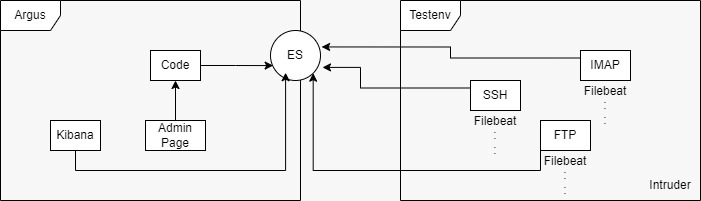
\includegraphics[width=\textwidth]{./images/concept.jpg}
        \caption{Concept Diagram of the Monitoring System \& Testing Environment}\label{fig:concept-diagram}
    \end{figure}

    \newpage
    \subsection{Requirements}\label{subsec:requirements}

    A comprehensive understanding of the project's requirements is essential for its success.
    This section details the functional and non-functional requirements, along with the criteria for defining and identifying malicious IP addresses.

    \subsubsection{Functional Requirements}\label{subsubsec:functional-requirements}

    Functional requirements define specific behaviors and functionalities that the system must perform.
    These requirements ensure that the system delivers the intended value and meets user expectations.

    \paragraph{Real-time Monitoring}
    \begin{itemize}
        \item Implement continuous monitoring of network traffic to identify unauthorized activities.
        \item Utilize system logs to detect patterns of malicious behavior, such as frequent login failures, port scanning, and abnormal traffic surges.
    \end{itemize}

    \paragraph{Automated Threat Detection}
    \begin{itemize}
        \item Develop algorithms capable of analyzing network traffic to flag potentially harmful IP addresses.
        \item Establish clear guidelines for identifying malicious activity, focusing on SSH, FTP, and IMAPS protocols.
    \end{itemize}

    \paragraph{Integration with AbuseIPDB}
    \begin{itemize}
        \item Connect with the AbuseIPDB API to report identified malicious IP addresses.
        \item Ensure the system continuously shares threat intelligence with AbuseIPDB to maintain updated data on malicious activities.
    \end{itemize}

    \paragraph{Alerting and Notification}
    \begin{itemize}
        \item Create a notification system to alert administrators of detected threats in real-time.
    \end{itemize}

    \paragraph{Comprehensive Reporting}
    \begin{itemize}
        \item Develop tools to generate detailed reports on network security events, traffic patterns, and system performance.
        \item Ensure reports are user-friendly and provide actionable insights for administrators.
    \end{itemize}

    \paragraph{User-friendly Interface}
    \begin{itemize}
        \item Design an intuitive web-based interface for administrators to manage and monitor network security.
        \item Include real-time visualizations of network traffic and threats, leveraging tools like Kibana for better user experience.
    \end{itemize}

    \paragraph{Scalability and Performance}
    \begin{itemize}
        \item Ensure the system can scale to monitor numerous servers and handle high traffic volumes efficiently.
        \item Optimize system components for minimal resource consumption while maintaining performance.
    \end{itemize}

    \paragraph{Documentation and Community Engagement}
    \begin{itemize}
        \item Provide comprehensive and regularly updated documentation for users and developers.
        \item Promote community involvement by making the project open-source.
        \item Encourage contributions and feedback from a community of users and developers to continually improve the system.
    \end{itemize}

    \subsubsection{Non-functional Requirements}\label{subsubsec:non-functional-requirements}

    Non-functional requirements impose constraints on the design or implementation, ensuring the system's performance, security, and reliability.

    \paragraph{Performance Requirements}
    \begin{itemize}
        \item The system shall process log data and generate alerts within 5 seconds of detecting suspicious activity.
    \end{itemize}

    \paragraph{Security Requirements}
    \begin{itemize}
        \item Data in transit shall be encrypted using TLS to prevent interception.
        \item Authentication and authorization mechanisms shall be implemented to restrict access to sensitive data and functionalities.
    \end{itemize}

    \subsubsection{Boundary and Pre-Conditions}\label{subsubsec:boundary-preconditions}

    The system must operate under specific boundary conditions and pre-conditions to ensure its effectiveness and compatibility with the existing infrastructure.
    These conditions outline the environment and prerequisites necessary for the successful deployment and operation of the monitoring system.

    \paragraph{Operating System}
\begin{itemize}
\item The system is designed to run on Ubuntu 20.04 or newer, with a focus on the amd64 architecture, ensuring full compatibility and optimal performance for the deployment of Docker containers and other system components.
\item While the project also supports the arm64 architecture, additional configuration steps may be necessary to ensure proper functionality. Users running the project on arm64 should refer to the provided documentation for specific setup instructions.
\item Running the project on other platforms is possible, but users may encounter compatibility issues, particularly with different architectures. Testing and adjustments may be required to ensure proper functionality on non-Ubuntu systems.
\item Users are encouraged to use Ubuntu 20.04 or newer on amd64 to avoid potential compatibility issues and to benefit from the extensive documentation and community support available for this operating system.
\item For other Linux distributions, as well as macOS and Windows, additional configuration steps might be necessary, particularly concerning Docker and system dependencies.
\end{itemize}

    \paragraph{Hardware Requirements}
    \begin{itemize}
        \item Adequate hardware resources must be available to handle monitoring and data processing tasks.
        This includes sufficient CPU, memory, and storage capacity to support the operation of Elasticsearch, Kibana, Filebeat, and custom scripts for threat detection and analysis.
    \end{itemize}

    \paragraph{Network Configuration}
    \begin{itemize}
        \item Proper network configurations must be in place to allow monitoring and traffic analysis.
        This includes configuring network interfaces, firewalls, and ensuring that necessary ports are open for communication between system components and external services.
        \item Ensure that the monitoring system can access and monitor network traffic on the specified ports and protocols (e.g., SSH, FTP, IMAPS).
    \end{itemize}

    \paragraph{Access Permissions}
    \begin{itemize}
        \item Necessary access permissions must be granted to monitor network traffic and system logs.
        This includes permissions to read log files, access network interfaces, and communicate with external APIs such as AbuseIPDB\@.
        \item System administrators must have sufficient privileges to configure and manage the monitoring system, including setting up Docker containers and managing Elasticsearch and Kibana instances.
    \end{itemize}

    \paragraph{Software Dependencies}
    \begin{itemize}
        \item The system relies on specific software dependencies, including Docker, Elasticsearch, Kibana, and Filebeat.
        Ensure that these dependencies are installed and properly configured on the host system.
        \item Custom scripts for threat detection and analysis must be compatible with the installed software versions and the overall system architecture.
    \end{itemize}

    \paragraph{Security Considerations}
    \begin{itemize}
        \item Data in transit must be encrypted using TLS to prevent interception and ensure the confidentiality and integrity of the monitored data.
        \item Authentication and authorization mechanisms must be in place to restrict access to sensitive data and functionalities.
        This includes securing access to the monitoring dashboard, Elasticsearch, and Kibana.
    \end{itemize}

    \paragraph{Integration with External Services}
    \begin{itemize}
        \item Integration with external services such as AbuseIPDB requires valid API keys and network access to the respective service endpoints.
        \item Ensure that the system can communicate with AbuseIPDB for real-time threat intelligence sharing and automated reporting of malicious IP addresses.
    \end{itemize}

    \paragraph{User Training and Documentation}
    \begin{itemize}
        \item System administrators and IT security teams must be adequately trained to use the monitoring system.
        This includes understanding how to configure and manage the system, interpret alerts and reports, and respond to detected threats.
        \item Comprehensive and up-to-date documentation must be provided to guide users through the setup, configuration, and operation of the monitoring system.
    \end{itemize}

    \noindent By adhering to these boundary conditions and pre-conditions, the monitoring system can be effectively deployed and operated, ensuring it meets the specified functional and non-functional requirements.

    \subsubsection{Characteristics of Malicious IP Addresses}\label{subsubsec:malicious-ip-characteristics}

    Malicious IP addresses are identified based on behaviors and activities that pose threats to system security.
    These characteristics include:

    \begin{itemize}
        \item \textbf{Unauthorized Access Attempts:} Malicious IPs frequently attempt to gain unauthorized access to systems.
        \item \textbf{Abnormal Traffic Patterns:} Malicious IPs often exhibit unusual traffic behaviors, such as port scanning and traffic spikes.
        \item \textbf{Failed Login Attempts:} A high number of consecutive failed login attempts can signal an IP engaged in unauthorized access attempts.
        \item \textbf{Known Malicious Activity:} IPs previously reported or flagged for malicious activities are often included in blacklists and reputation services.
        \item \textbf{Suspicious Transfers:} Unusual data transfer activities can indicate malicious intent.
    \end{itemize}

    \subsubsection{Implementation Details}\label{subsubsec:implementation-details}

    Our project focuses on monitoring and detecting the following specific types of malicious activities:

    \begin{itemize}
        \item \textbf{Brute Force Attacks:} Detects continuous, rapid attempts to guess passwords or credentials by monitoring for more than five login attempts within ten seconds.
        Each detected brute force attack triggers an alert and logs the incident for further analysis.
        \item \textbf{Port Scanning:} Identifies probing for open ports by monitoring for sequential access attempts to different ports within a short time frame.
        Each port scanning activity is logged, and an alert is generated.
        \item \textbf{Traffic Spikes:} Detects sudden, significant increases in traffic by comparing current traffic levels to historical baselines.
        A spike exceeding predefined thresholds will trigger an alert and be logged for further investigation.
        \item \textbf{Failed Login Attempts:} Monitors for excessive failed login attempts by tracking the number of consecutive failures.
        More than five failed attempts within a specific time window will trigger an alert and log the incident.
        \item \textbf{Known Malicious Activity:} Cross-references incoming IP addresses with databases like AbuseIPDB to identify IPs known for malicious behavior.
        Each match generates an alert and logs the activity.
        \item \textbf{Suspicious Transfers:} Monitors for large or unusual data transfers by analyzing transfer volumes and patterns.
        Transfers significantly deviating from the norm trigger an alert and are logged.
    \end{itemize}

    \subsubsection{Consideration of IP Subnets}\label{subsubsec:ip-subnets}

    Our system focuses on identifying and reporting individual malicious IP addresses rather than blocking entire IP subnets.
    Blocking full subnets can lead to significant collateral damage, potentially restricting access for legitimate users sharing the same subnet.
    However, depending on community demands, we might implement this feature or provide guidelines on how to implement it for administrators in their environments.

    \begin{itemize}
        \item \textbf{Impact Assessment:} Evaluate the potential impact on legitimate users before implementing subnet blocking.
        \item \textbf{Guidelines:} Provide detailed guidelines for administrators on how to configure subnet blocking if deemed necessary for their specific environments.
    \end{itemize}

    \subsubsection{Manual Review and No Automated Blocking}\label{subsubsec:manual-review}
    We have chosen not to implement automated IP blocking, such as updating IP-tables rules, within this system.
    Automated blocking can lead to false positives and unintentional disruptions.
    Instead, all detected threats are reported to the system administrator for manual review and verification.\\

    \noindent By focusing on these specific activities and incorporating manual review processes, our system aims to provide accurate and actionable threat intelligence while maintaining flexibility and minimizing the risk of unnecessary disruptions.

    \subsection{Usability}\label{subsec:usability}

    \subsubsection{Personas}\label{subsubsec:personas}
    The primary users of this monitoring system are diverse, each with unique roles and responsibilities.
    Understanding these personas helps tailor the system to meet their specific needs.

    \begin{itemize}
        \item \textbf{System Administrators:}
        \begin{itemize}
            \item \textbf{Responsibilities:} Managing and maintaining the IT infrastructure, ensuring system security, and responding to alerts.
            \item \textbf{Needs:} Comprehensive dashboard for real-time monitoring, detailed logs for troubleshooting, and tools for quick response to incidents.
            \item \textbf{Challenges:} Handling a wide range of systems and services, managing alerts from various sources, and maintaining system uptime and security.
        \end{itemize}

        \item \textbf{IT Security Teams:}
        \begin{itemize}
            \item \textbf{Responsibilities:} Monitoring, detecting, and mitigating security threats across the organization's network.
            \item \textbf{Needs:} Advanced analytics for threat detection, integration with threat intelligence services, and capabilities for detailed incident investigation.
            \item \textbf{Challenges:} Staying ahead of evolving threats, managing large volumes of security data, and coordinating responses to incidents.
        \end{itemize}

        \item \textbf{Network Engineers:}
        \begin{itemize}
            \item \textbf{Responsibilities:} Designing, implementing, and maintaining network infrastructure.
            \item \textbf{Needs:} Visibility into network traffic patterns, tools for diagnosing network issues, and insights into potential network vulnerabilities.
            \item \textbf{Challenges:} Ensuring network performance and reliability, managing network security, and responding to network-related incidents.
        \end{itemize}

        \item \textbf{Compliance Officers:}
        \begin{itemize}
            \item \textbf{Responsibilities:} Ensuring the organization adheres to regulatory requirements and industry standards.
            \item \textbf{Needs:} Audit trails for security events, compliance reports, and tools for monitoring compliance with security policies.
            \item \textbf{Challenges:} Keeping up with changing regulations, ensuring compliance across the organization, and managing compliance documentation.
        \end{itemize}

        \item \textbf{Executive Management:}
        \begin{itemize}
            \item \textbf{Responsibilities:} Overseeing the overall security posture of the organization and making strategic decisions.
            \item \textbf{Needs:} High-level reports on security metrics, insights into major security incidents, and information on the effectiveness of security controls.
            \item \textbf{Challenges:} Balancing security with business objectives, allocating resources effectively, and understanding complex security issues.
        \end{itemize}
    \end{itemize}

    \subsection{Storyboard}\label{subsec:storyboard}
    The storyboard illustrates typical scenarios where various stakeholders interact with the monitoring system:

    \subsubsection{User Scenarios}\label{subsubsec:user-scenarios}

    \begin{itemize}
        \item \textbf{Scenario 1: Real-time Alert Response}
        \begin{itemize}
            \item An IT security analyst receives a real-time alert about a suspicious IP address attempting to access the server via SSH\@.
            \item The analyst logs into the monitoring dashboard, reviews the alert details, and identifies the malicious IP address.
            \item The analyst informs the system administrator to take appropriate action, such as blocking the IP address and reporting it to AbuseIPDB\@.
        \end{itemize}

        \item \textbf{Scenario 2: Daily Security Review}
        \begin{itemize}
            \item IT security teams review daily reports generated by the monitoring system, summarizing detected threats and network activity.
            \item The team analyzes trends and patterns to identify potential vulnerabilities and plan for preventive measures.
            \item Reports are shared with relevant stakeholders, including compliance officers and executive management, to keep them informed about the security posture of the organization.
        \end{itemize}

        \item \textbf{Scenario 3: Investigating Suspicious Activity}
        \begin{itemize}
            \item A security analyst notices unusual traffic patterns in the network logs visualized in the dashboard.
            \item The analyst drills down into the data to investigate specific IP addresses, connection attempts, and failure logs.
            \item Based on the findings, the analyst recommends specific actions to the IT team, such as tightening firewall rules or conducting a deeper forensic analysis.
        \end{itemize}

        \item \textbf{Scenario 4: Reporting a False Positive}
        \begin{itemize}
            \item An IP address is flagged as suspicious due to multiple failed login attempts, but the network engineer realizes it's a legitimate user who mistyped their password.
            \item The engineer accesses the dashboard, reviews the activity logs, and verifies the user's identity.
            \item The engineer marks the alert as a false positive and updates the system to prevent similar alerts in the future.
        \end{itemize}

        \item \textbf{Scenario 5: System Maintenance and Updates}
        \begin{itemize}
            \item The IT team plans a maintenance window to update the monitoring system and its dependencies.
            \item Before the maintenance begins, the team reviews the current system status and schedules the update during off-peak hours.
            \item Post-maintenance, the team verifies the integrity of the monitoring system, ensuring all components are functioning correctly and logs are being accurately collected and analyzed.
        \end{itemize}

        \item \textbf{Scenario 6: Training New Administrators}
        \begin{itemize}
            \item A new system administrator joins the IT team and needs to be trained on using the monitoring system.
            \item The experienced team members provide a walkthrough of the dashboard, explain the key functionalities, and demonstrate how to respond to alerts.
            \item The new administrator practices handling mock alerts and reviewing reports to become proficient in using the system.
        \end{itemize}

        \item \textbf{Scenario 7: Executive Management Review}
        \begin{itemize}
            \item Executive management reviews high-level reports on security metrics, including major incidents and the effectiveness of security controls.
            \item They use these insights to make strategic decisions regarding resource allocation and overall security strategy.
            \item Management coordinates with the IT security team to address any identified gaps or areas for improvement.
        \end{itemize}

        \item \textbf{Scenario 8: Compliance Audit}
        \begin{itemize}
            \item Compliance officers conduct an audit of security events and incident responses to ensure regulatory requirements are met.
            \item They access detailed logs and audit trails provided by the monitoring system.
            \item The officers prepare compliance reports and recommend policy updates based on audit findings.
        \end{itemize}
    \end{itemize}

    \subsection{UX-Prototyping}\label{subsec:ux-prototyping}

    Prototype designs for the user interface are focused on ensuring ease of use and accessibility, even for non-technical users.
    The system will come with a fully functional UI that displays basic analysis, but for implementation in a productive environment, the system administrator will likely need to customize it based on the specific services they want to monitor.

    \subsubsection{Kibana Monitoring System}\label{subsubsec:kibana-monitoring-system}

    The Kibana monitoring system provides real-time visualization and analysis of network activity and detected threats.
    This interface is designed for system administrators to monitor the overall health and security status of their systems effectively.

    \begin{itemize}
        \item \textbf{Intuitive Dashboard:} The Kibana dashboard offers a clear and interactive overview of network activity, detected threats, and system performance.
        \item \textbf{Customizable Views:} Administrators can create and customize their dashboards to focus on specific metrics and logs that are most relevant to their security needs.
        \item \textbf{Real-Time Visualizations:} Provides real-time visualizations, including graphs, charts, and alerts, to help administrators quickly identify and respond to security incidents.
        \item \textbf{Detailed Log Information:} Allows in-depth analysis of log data with filtering, searching, and drilling down into specific events.
    \end{itemize}

    \noindent  It is important to note that designing a static UI interface for Kibana does not make practical sense, as users will inevitably need to customize and modify their dashboards to meet their unique monitoring requirements.
    Kibana’s flexibility and powerful customization options are key features that enable users to tailor their monitoring setup dynamically.

    \subsubsection{Web-Based Admin Interface}\label{subsubsec:web-based-admin-interface}

    The web-based admin interface is designed for system administrators to manage and report suspicious IP addresses.
    This interface facilitates easy navigation and quick actions for reporting detected threats to external services such as AbuseIPDB\@.

    \begin{itemize}
        \item \textbf{Suspicious IP Address List:} Displays a list of detected suspicious IP addresses along with the number of failed login attempts and the timestamp of the last attempted login.
        \item \textbf{Report Functionality:} Provides a "Report" button next to each suspicious IP address, allowing administrators to quickly report these IPs to AbuseIPDB\@.
        \item \textbf{User-Friendly Navigation:} The interface is designed to be straightforward, with clear labels and workflows that guide administrators through the process of managing and reporting threats.
    \end{itemize}

    \begin{figure}[H]
        \centering
        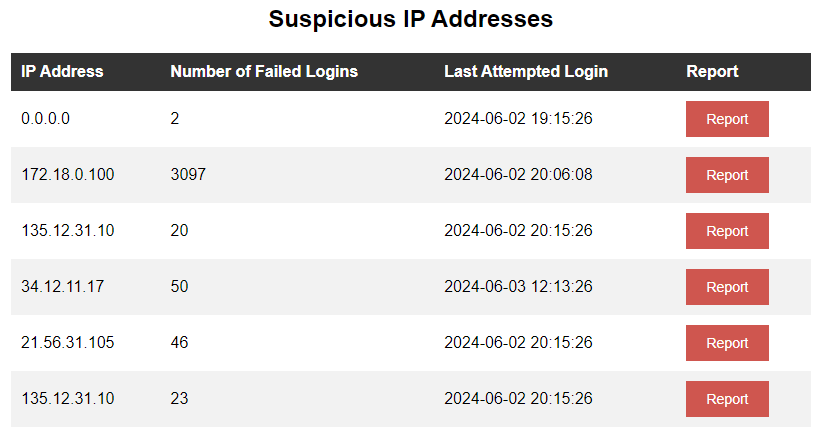
\includegraphics[width=\textwidth]{./images/mockup.png}
        \caption{System Administrator Interface Mockup}
        \label{fig:sysadmin-interface}
    \end{figure}

    \newpage
% Implementation


    \section{Implementation}\label{sec:implementation}

    \subsection{Architecture}\label{subsec:architecture}

    The architecture of our system is divided into two main components: the monitoring environment (Argus) and the testing environment.
    This section outlines the components and interactions within these environments based on the provided file structure.

    \subsubsection{Argus (Monitoring Environment)}\label{subsubsec:argus-environment}

    The Argus environment is responsible for monitoring, analyzing, and reporting malicious activities within the network.
    The primary components include:

    \paragraph{File Structure Overview:}
    \begin{itemize}
        \item \textbf{argus/} - Contains the main monitoring scripts and configurations.
        \begin{itemize}
            \item \texttt{shared-data/} - Directory for shared data.
            \item \texttt{abuseIPDB.py} - Script for interacting with AbuseIPDB.
            \item \texttt{monitor.py} - Main monitoring script.
            \item \texttt{brute\_force.py, port\_scanning.py, suspicious\_transfers.py, traffic\_spikes.py} - Supporting scripts for specific detection algorithms.
        \end{itemize}
        \item \textbf{elasticsearch/} - Contains Elasticsearch configuration.
        \begin{itemize}
            \item \texttt{config/elasticsearch.yml} - Configuration file for Elasticsearch.
        \end{itemize}
        \item \textbf{kibana/} - Configuration and Docker setup for Kibana.
        \begin{itemize}
            \item \texttt{kibana.yml} - Configuration file for Kibana.
        \end{itemize}
        \item \textbf{webapp/} - Contains the web application for reporting suspicious IPs.
        \begin{itemize}
            \item \texttt{templates/} - HTML templates for the web application.
            \item \texttt{app.py} - Main Flask application script.
            \item \texttt{Dockerfile} - Dockerfile for setting up the web application.
        \end{itemize}
        \item \texttt{docker-compose.yml} - Docker Compose file to orchestrate the deployment of all services.
    \end{itemize}

    \paragraph{Components and Functions:}
    \begin{itemize}
        \item \textbf{Docker Engine:} Provides the containerization platform for deploying various services.
        Docker ensures that the system components are modular and can be easily managed and scaled.
        \item \textbf{Filebeat:} Installed on monitored servers to collect and ship log data to Elasticsearch.
        Filebeat efficiently forwards logs, ensuring minimal latency and loss.
        \item \textbf{Elasticsearch:} A distributed, RESTful search and analytics engine used for storing and indexing log data for analysis.
        Elasticsearch enables fast search responses, making real-time data analysis feasible.
        \item \textbf{Kibana:} Provides visualization capabilities for log data and a web-based interface for administrators.
        Kibana allows for the creation of dashboards that display real-time monitoring data.
        \item \textbf{Argus Scripts:} Custom scripts (e.g., \texttt{monitor.py}, \texttt{brute\_force.py}, \texttt{port\_scanning.py}) analyze log data to identify suspicious patterns and potential security threats.
    \end{itemize}

    \paragraph{Data Flow:}
    \begin{itemize}
        \item Filebeat collects logs from monitored servers (SSH, FTP, IMAPS) and forwards them to Elasticsearch.
        \item Elasticsearch indexes the collected log data, enabling efficient search and analysis.
        \item Argus scripts analyze the indexed data to identify suspicious activities such as brute force attacks, port scanning, and unusual traffic spikes.
        \item Detected threats are visualized on Kibana dashboards and reported to administrators through the web application.
        \item Integration with AbuseIPDB is achieved through \texttt{abuseIPDB.py} for reporting malicious IPs.
    \end{itemize}

    \subsubsection{Testing Environment Implementation}\label{subsubsec:testing-environment-implementation}

    The testing environment simulates real-world scenarios to validate the functionality and effectiveness of the Argus monitoring system.
    The primary components include:

    \paragraph{File Structure Overview:}
    \begin{itemize}
        \item \textbf{ftp\_server/} - Configuration and Docker setup for the FTP server.
        \begin{itemize}
            \item \texttt{Dockerfile} - Dockerfile for setting up the FTP server.
            \item \texttt{filebeat.yml} - Configuration for Filebeat on the FTP server.
        \end{itemize}
        \item \textbf{mail\_server/} - Configuration and Docker setup for the IMAPS server.
        \begin{itemize}
            \item \texttt{Dockerfile} - Dockerfile for setting up the mail server.
            \item \texttt{filebeat.yml} - Configuration for Filebeat on the mail server.
        \end{itemize}
        \item \textbf{ssh\_server/} - Configuration and Docker setup for the SSH server.
        \begin{itemize}
            \item \texttt{Dockerfile} - Dockerfile for setting up the SSH server.
            \item \texttt{filebeat.yml} - Configuration for Filebeat on the SSH server.
        \end{itemize}
        \item \textbf{intruder/} - Contains the intruder simulation scripts.
        \begin{itemize}
            \item \texttt{Dockerfile} - Dockerfile for setting up the intruder environment.
            \item \texttt{intruder.sh} - Script for simulating intruder activities.
        \end{itemize}
    \end{itemize}

    %uml diagram
    \begin{figure}[H]
        \centering
        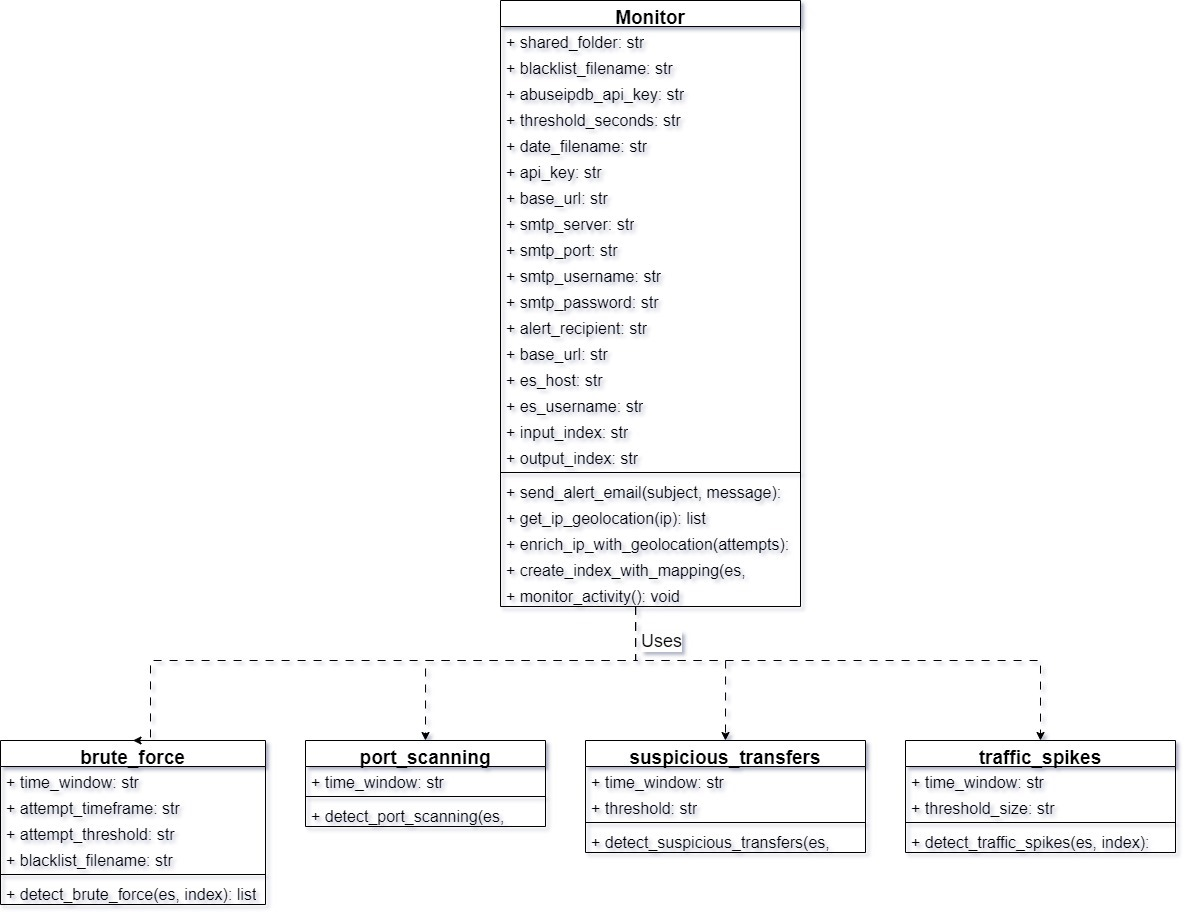
\includegraphics[width=\textwidth]{./images/uml.jpg}
        \caption{UML Class Diagram of the System Environment}
        \label{fig:uml_diagram}
    \end{figure}

    \paragraph{Components and Functions:}
    \begin{itemize}
        \item \textbf{SSH Server:} Simulates an SSH service to monitor and detect unauthorized access attempts.
        \item \textbf{FTP Server:} Simulates an FTP service to monitor and detect unauthorized file transfer attempts.
        \item \textbf{IMAPS Server:} Simulates an IMAPS service to monitor and detect unauthorized email access attempts.
        \item \textbf{Intruder Simulation:} The \texttt{intruder.sh} script simulates attacks such as brute force, port scanning, and suspicious data transfers to test the effectiveness of the Argus monitoring system.
    \end{itemize}

    \newpage
    \paragraph{Data Flow:}
    \begin{itemize}
        \item The intruder simulation script generates malicious activities targeting the SSH, FTP, and IMAPS servers.
        \item Filebeat on each server collects logs of these activities and forwards them to Elasticsearch in the monitoring environment.
        \item Argus scripts analyze the logs in Elasticsearch to detect the simulated attacks.
        \item Detection results are visualized in Kibana and can be acted upon by administrators using the web application.
    \end{itemize}

    \begin{figure}[H]
        \centering
        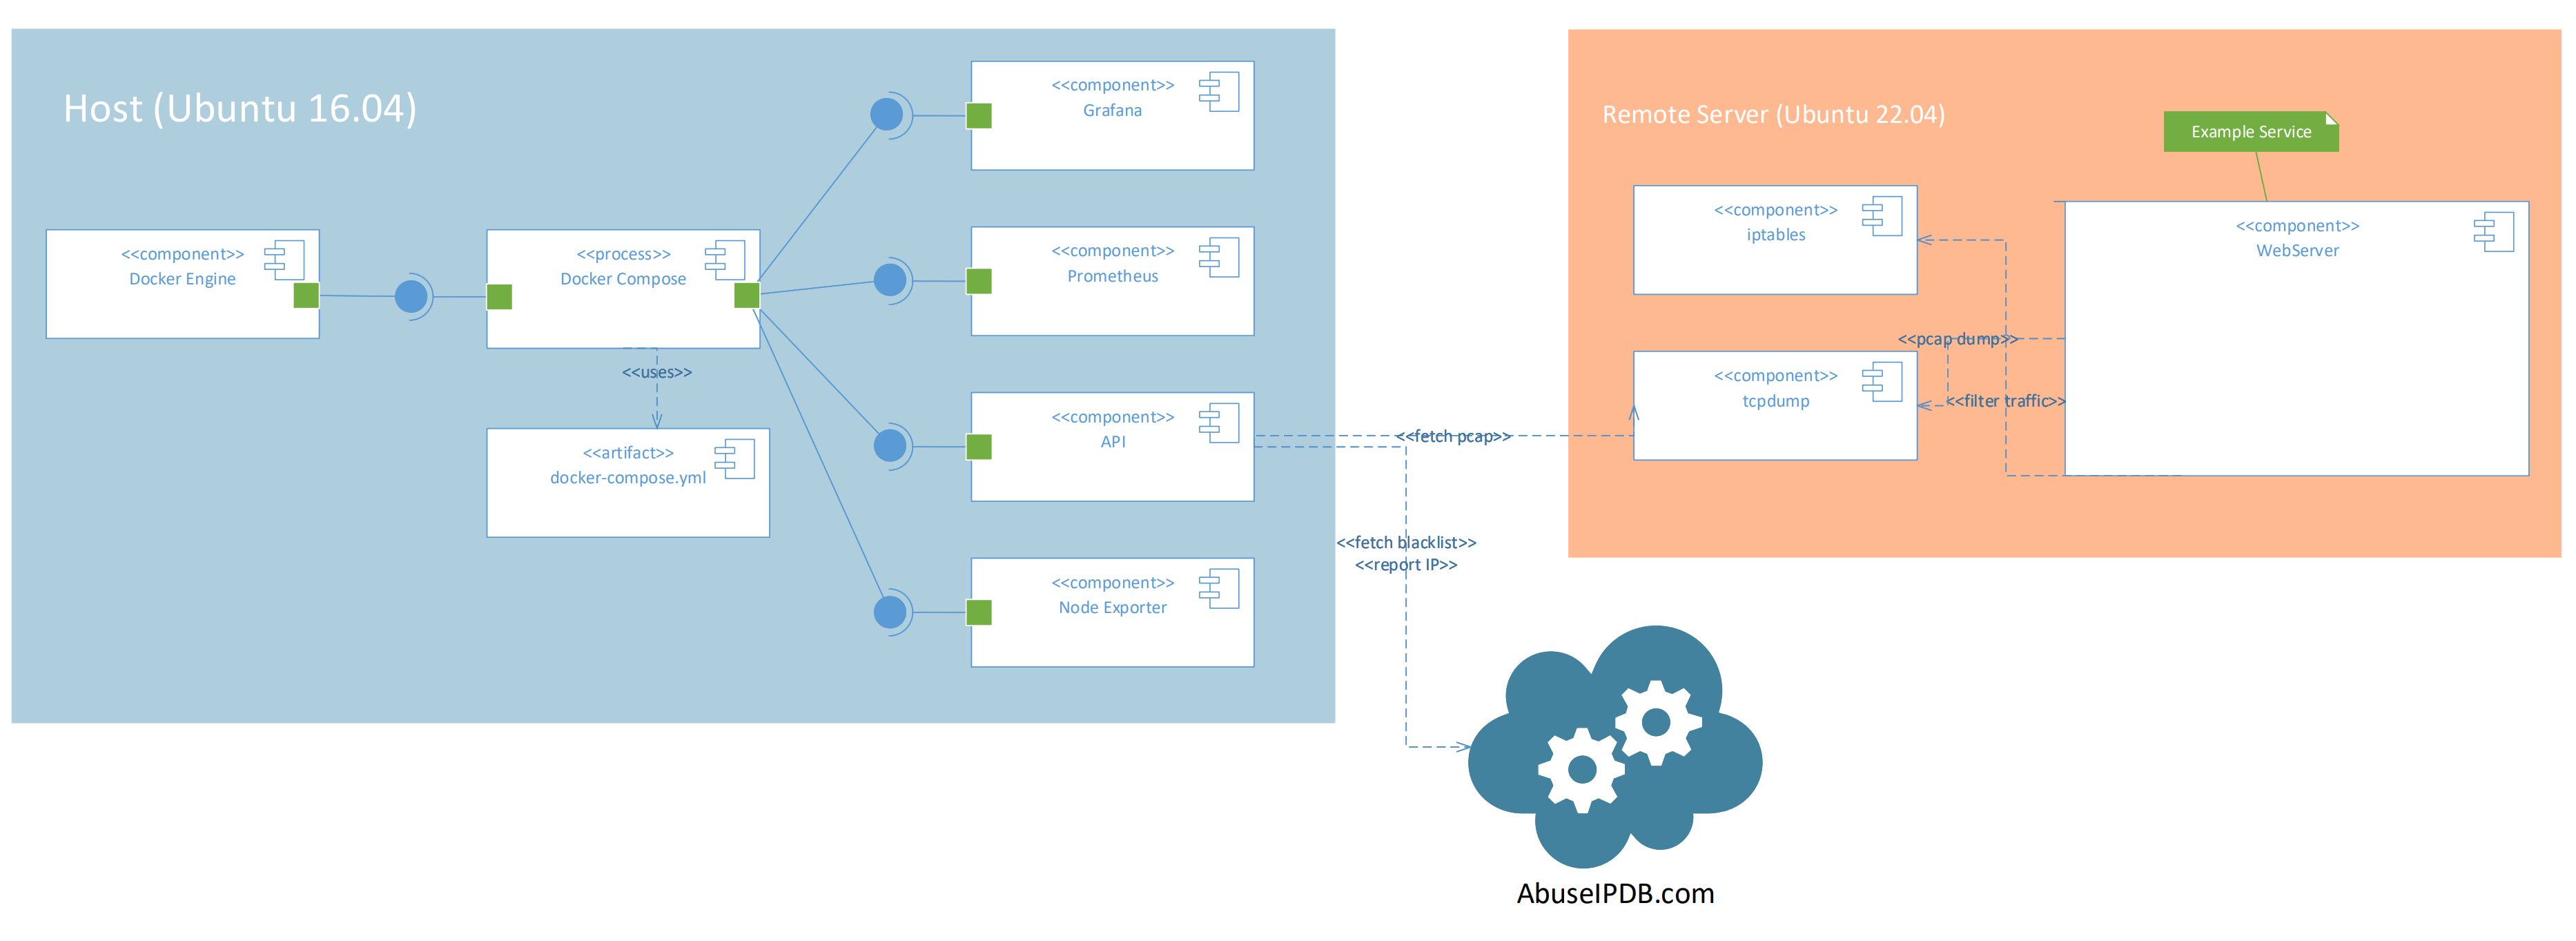
\includegraphics[width=\textwidth]{./images/component.png}
        \caption{Component Diagram of the System Environment}
        \label{fig:component_diagram}
    \end{figure}

    \noindent The implementation is carried out using Python, following the PEP 8 coding guidelines to ensure code readability and maintainability.

    \newpage
    \subsection{Processes}\label{subsec:processes}

    This subsection details the methodologies and frameworks used to manage the project, ensuring it is delivered on time and meets the required standards.

    \subsubsection{SCRUM Framework}

    The Scrum framework was essential in managing the project's complex software development processes, emphasizing teamwork, accountability, and iterative progress.
    The key components of our Scrum process included:

    \paragraph{Roles:}
    \begin{itemize}
        \item \textbf{Product Owner:} Rezzonico Marco - Responsible for maximizing the value of the product and managing the Product Backlog.
        \item \textbf{Scrum Master:} Pelletier Max - Facilitates Scrum practices and ensures the team adheres to Scrum principles.
        \item \textbf{Development Team:} Pernjak Stefani, Pelletier Max, Rezzonico Marco - Responsible for delivering potentially shippable increments of the product at the end of each Sprint.
    \end{itemize}

    \paragraph{Events:}
    \begin{itemize}
        \item \textbf{Sprint Planning:} Held at the start of each two-week sprint cycle, defining the work scope and objectives.
        \item \textbf{Daily Stand-Ups:} Short, daily meetings to align on project progress and address concerns.
        \item \textbf{Sprint Review:} Meeting held at the end of each sprint to present completed work to stakeholders and gather feedback.
        \item \textbf{Sprint Retrospective:} Meeting held after the Sprint Review to reflect on the sprint process.
    \end{itemize}

    \paragraph{Artifacts:}
    \begin{itemize}
        \item \textbf{Product Backlog:} Managed in Jira, it is continuously updated and prioritized by the Product Owner.
        \item \textbf{Sprint Backlog:} A subset of the Product Backlog items selected for the sprint.
        \item \textbf{Increment:} The sum of all the Product Backlog items completed during a sprint.
    \end{itemize}

    \noindent For the detailed Scrum Reports, please refer to the \texttt{ScrumReport} directory.

    \subsubsection{Project Management Tools}

    The project management tools used to facilitate communication, collaboration, and task tracking included:

    \begin{itemize}
        \item \textbf{Jira:} Used for managing the Product Backlog, Sprint Backlog, and tracking progress on tasks.
        \item \textbf{GitLab:} For version control, code collaboration, and managing project repositories.
        \item \textbf{MS-Teams:} For real-time communication, meetings, and collaboration among team members.
    \end{itemize}

    \subsubsection{Additional Processes}

    \paragraph{Definition of Ready:}
    A user story or task must meet specific criteria to be considered \textit{Ready} for inclusion in a sprint, including clearly defined user stories, specified acceptance criteria, identified dependencies, and no blocking issues.

    \paragraph{Definition of Done:}
    For a task within a sprint to be considered \textit{Done}, it must satisfy criteria such as complete code implementation, peer review, successful testing, updated documentation, and deployment readiness.

    \subsubsection{Sprint Goals}

    \paragraph{Sprint 1: Initial Setup and Research}
    \begin{itemize}
        \item \textbf{Goal:} Establish development environment and conduct initial research.
        \item \textbf{Tasks:}
        \begin{itemize}
            \item Set up development environments on team members' machines.
            \item Research existing tools and technologies for IP monitoring.
            \item Gather requirements and define initial project scope.
        \end{itemize}
        \item \textbf{Deliverables:}
        \begin{itemize}
            \item Fully configured development environment.
            \item Research documentation outlining tools, technologies, and best practices.
            \item Initial project scope document.
        \end{itemize}
    \end{itemize}

    \paragraph{Sprint 2: Basic Monitoring Implementation}
    \begin{itemize}
        \item \textbf{Goal:} Implement basic IP monitoring functionality.
        \item \textbf{Tasks:}
        \begin{itemize}
            \item Develop a basic script to monitor IP addresses.
            \item Test the script on local environments.
            \item Begin documentation for the monitoring script.
        \end{itemize}
        \item \textbf{Deliverables:}
        \begin{itemize}
            \item Basic IP monitoring script.
            \item Initial test results demonstrating script functionality.
            \item Draft of script documentation.
        \end{itemize}
    \end{itemize}

    \paragraph{Sprint 3: Integration with AbuseIPDB}
    \begin{itemize}
        \item \textbf{Goal:} Integrate monitoring with AbuseIPDB for reporting.
        \item \textbf{Tasks:}
        \begin{itemize}
            \item Integrate the basic monitoring script with AbuseIPDB API\@.
            \item Test integration by reporting suspicious IPs to AbuseIPDB\@.
            \item Update documentation to include integration steps.
        \end{itemize}
        \item \textbf{Deliverables:}
        \begin{itemize}
            \item Integrated monitoring script with AbuseIPDB\@.
            \item Test reports showcasing successful AbuseIPDB integration.
            \item Updated documentation with integration details.
        \end{itemize}
    \end{itemize}

    \paragraph{Sprint 4: Traffic Monitoring}
    \begin{itemize}
        \item \textbf{Goal:} Implement live traffic monitoring with iptables.
        \item \textbf{Tasks:}
        \begin{itemize}
            \item Develop a script to monitor live traffic using iptables.
            \item Test the script on a controlled environment to ensure accuracy.
            \item Document the setup and usage of the traffic monitoring script.
        \end{itemize}
        \item \textbf{Deliverables:}
        \begin{itemize}
            \item Live traffic monitoring script using iptables.
            \item Test logs demonstrating the effectiveness of the traffic monitoring.
            \item Documentation for traffic monitoring setup and usage.
        \end{itemize}
    \end{itemize}

    \paragraph{Sprint 5: Malicious Traffic Definition}
    \begin{itemize}
        \item \textbf{Goal:} Establish criteria for malicious traffic (SSH, SFTP, IMAPS).
        \item \textbf{Tasks:}
        \begin{itemize}
            \item Define specific criteria for identifying malicious traffic for different protocols.
            \item Implement scripts to detect and log malicious traffic based on defined criteria.
            \item Develop a mechanism for \("\)shaming\("\) bad actors by logging and reporting their IP addresses.
        \end{itemize}
        \item \textbf{Deliverables:}
        \begin{itemize}
            \item Documented criteria for identifying malicious traffic.
            \item Implemented scripts for detecting malicious traffic.
            \item Logs and reports shaming bad actors.
        \end{itemize}
    \end{itemize}

    \paragraph{Sprint 6: Alerting and Reporting}
    \begin{itemize}
        \item \textbf{Goal:} Set up alerting and develop reporting tools.
        \item \textbf{Tasks:}
        \begin{itemize}
            \item Implement an alerting system for detected malicious traffic.
            \item Develop tools for generating detailed reports for system administrators.
            \item Prepare and finalize the project presentation.
        \end{itemize}
        \item \textbf{Deliverables:}
        \begin{itemize}
            \item Functional alerting system.
            \item Reporting tools for system administrators.
            \item Final project presentation.
        \end{itemize}
    \end{itemize}

    \paragraph{Sprint 7: Final Adjustments and Presentation}
    \begin{itemize}
        \item \textbf{Goal:} Refine the monitoring system, enhance alerting mechanisms, and finalize documentation and presentation.
        \item \textbf{Tasks:}
        \begin{itemize}
            \item Review and optimize the existing monitoring and alerting scripts based on the latest test results.
            \item Conduct a thorough system audit to ensure all components are functioning as expected.
            \item Finalize and compile all project documentation, including user manuals, technical documentation, and deployment guides.
            \item Prepare and polish the final presentation to showcase the project.
        \end{itemize}
        \item \textbf{Deliverables:}
        \begin{itemize}
            \item Optimized monitoring and alerting scripts.
            \item Complete and polished final documentation.
            \item Final presentation.
        \end{itemize}
    \end{itemize}

    \paragraph{Sprint 8: Final Testing and Deployment}
    \begin{itemize}
        \item \textbf{Goal:} Conduct final testing and prepare for deployment.
        \item \textbf{Tasks:}
        \begin{itemize}
            \item Perform end-to-end testing of the monitoring system.
            \item Address any remaining issues or bugs.
            \item Prepare deployment scripts and documentation.
        \end{itemize}
        \item \textbf{Deliverables:}
        \begin{itemize}
            \item Completed end-to-end testing results.
            \item Resolved issues and bugs.
            \item Deployment scripts and documentation.
        \end{itemize}
    \end{itemize}

    \newpage
% Deployment/Integration


    \section{Deployment/Integration}\label{sec:deployment-integration}

    \subsection{Licensing}\label{subsec:licensing}

    The Argus monitoring system is released under the GNU General Public License (GPL), version 3.
    This open-source license is designed to ensure that the software remains free and open, allowing users to run, study, share, and modify the software.
    The key aspects of the GNU GPL v3 include:

    \begin{itemize}
        \item \textbf{Freedom to Use:} Users have the freedom to use the software for any purpose.
        \item \textbf{Freedom to Study and Modify:} The source code is available for users to study how the program works and to modify it to suit their needs.
        \item \textbf{Freedom to Distribute Copies:} Users can redistribute copies of the original program to help others.
        \item \textbf{Freedom to Distribute Modified Versions:} Users can distribute copies of their modified versions to others.
        By doing so, they can give the whole community a chance to benefit from their changes.
    \end{itemize}

    \noindent The full text of the GNU General Public License, version 3, is available at the following link: \url{https://www.gnu.org/licenses/gpl-3.0.html}.\\

    \noindent Here is a brief summary of the license:

    \begin{quote}
        \textbf{GNU GENERAL PUBLIC LICENSE
        Version 3, 29 June 2007}

        The GNU General Public License is a free, copyleft license for software and other kinds of works.\\

        \noindent The licenses for most software and other practical works are designed to take away your freedom to share and change the works.
        By contrast, the GNU General Public License is intended to guarantee your freedom to share and change all versions of a program--to make sure it remains free software for all its users.
        We, the Free Software Foundation, use the GNU General Public License for most of our software; it applies also to any other work released this way by its authors.
        You can apply it to your programs, too.\\

        \noindent When we speak of free software, we are referring to freedom, not price.
        Our General Public Licenses are designed to make sure that you have the freedom to distribute copies of free software (and charge for them if you wish), that you receive source code or can get it if you want it, that you can change the software or use pieces of it in new free programs, and that you know you can do these things.\\

        \noindent To protect your rights, we need to prevent others from denying you these rights or asking you to surrender the rights.
        Therefore, you have certain responsibilities if you distribute copies of the software, or if you modify it: responsibilities to respect the freedom of others.\\

        \noindent For example, if you distribute copies of such a program, whether gratis or for a fee, you must pass on to the recipients the same freedoms that you received.
        You must make sure that they, too, receive or can get the source code.
        And you must show them these terms so they know their rights.
    \end{quote}

    \noindent For a comprehensive understanding of the GNU General Public License, please refer to the full document linked above.
    This license choice ensures that Argus remains a robust, community-driven project that benefits from widespread collaboration and transparency.

    \newpage
    \subsection{Deployment Guide}\label{subsec:deployment-guide}

    This deployment guide provides detailed steps for setting up our monitoring system project for testing purposes.
    This guide is intended for a controlled testing environment and is not intended for direct deployment in a production environment.

    \subsubsection{Preparation}\label{subsubsec:preparation}

    Before deploying the system, ensure the following system requirements are met and discuss the necessary details with your team:

    \paragraph{System Requirements:}
    \begin{itemize}
        \item \textbf{Operating System:} Ubuntu 20.04 or newer.
        \item \textbf{Hardware:} Sufficient CPU, RAM, and storage to handle monitoring and data processing tasks.
        \item \textbf{Network Configuration:} Properly configured network settings to allow traffic monitoring and analysis.
        \item \textbf{Access Permissions:} Necessary permissions to monitor network traffic and system logs.
    \end{itemize}

    \paragraph{Team Discussions:}
    \begin{itemize}
        \item \textbf{Definition of Malicious IPs:} Clearly define what constitutes a malicious IP address in your context, such as unauthorized access attempts, abnormal traffic patterns, and failed login attempts.
        \item \textbf{Testing Environment:} Decide if you want to run the test environment first to validate the system's functionality.
        This includes setting up testing servers (e.g., SSH, FTP, IMAPS) and the intruder simulator.
    \end{itemize}

    \subsubsection{Deployment Steps}\label{subsubsec:deployment-steps}

    Follow these steps to deploy the monitoring system and testing environment:

    \paragraph{1. Deploying the Monitoring System:}
    \begin{itemize}
        \item Install Docker and Docker Compose:
        \begin{itemize}
            \item \texttt{sudo apt install docker docker-compose}
        \end{itemize}
        \item Clone the project repository:
        \begin{itemize}
            \item \texttt{git clone https://gitlab.ti.bfh.ch/pellm4/argus}
            \item Navigate to the project directory: \texttt{cd argus}
        \end{itemize}
        \item Build the project:
        \begin{itemize}
            \item \texttt{docker-compose build}
        \end{itemize}
        \item Run the containers (note that this might use a lot of resources):
        \begin{itemize}
            \item \texttt{docker-compose up -d}
        \end{itemize}
        \item Configure Kibana:
        \begin{itemize}
            \item Access Kibana at \texttt{http://127.0.0.1:5601}
            \item Log in with username: \texttt{elastic} and password: \texttt{argusIsTheBest123}
            \item Navigate to Stack Management / Saved Objects
            \item Import the \texttt{argus/export.ndjson} file
            \item Choose "Automatically overwrite conflicts"
        \end{itemize}
        \item Elasticsearch is available at \texttt{http://127.0.0.1:9200} with the same username and password as Kibana.
        \item The Admin Interface to report malicious IPs is available at \texttt{http://127.0.0.1:5000}.
    \end{itemize}

    \subsubsection{Configuration and Verification}\label{subsubsec:config-verification}
    \begin{itemize}
        \item \textbf{Verify System Operation:}
        \begin{itemize}
            \item Monitor the log data in Elasticsearch to ensure logs are collected correctly.
            \item Verify that Kibana dashboards display real-time data and visualizations.
            \item Confirm that the web-based admin interface is operational and can report malicious IP addresses.
        \end{itemize}

        \item \textbf{Testing:}
        \begin{itemize}
            \item Perform end-to-end testing by simulating various attack scenarios using the intruder.
            \item Ensure that the system correctly identifies and reports malicious activities.
            \item Review logs and alerts to verify accuracy and completeness.
        \end{itemize}
    \end{itemize}

    \subsubsection{Post-Deployment Activities}\label{subsubsec:post-deployment}
    \begin{itemize}
        \item \textbf{Ongoing Monitoring and Maintenance:}
        \begin{itemize}
            \item Regularly monitor the system to ensure continuous operation.
            \item Perform routine maintenance and updates to keep the system secure and efficient.
            \item Adjust configurations as necessary to adapt to changing network conditions and threat landscapes.
        \end{itemize}
    \end{itemize}

    \noindent By following this guide, users can set up and validate the monitoring system in a controlled testing environment, ensuring it meets their specific requirements and integrates seamlessly into their existing infrastructure.

    \newpage
    \section{Conclusion}\label{sec:Conclusion}
    The Malicious IP-Address Monitor project has successfully developed a robust, open-source tool designed to enhance internet security by monitoring and reporting unauthorized system administration traffic on Linux servers.
    Our primary goal was to provide a free, efficient, and user-friendly solution to detect and report malicious IP addresses, and we have accomplished this with great success.
    This tool not only proves invaluable for individual system administrators but also serves as a critical asset for organizations striving to maintain secure server environments.\\

    \noindent Throughout the development process, we adhered to the best practices in software development, including comprehensive testing, incorporating user feedback, and making iterative improvements.
    The successful deployment on Ubuntu servers demonstrated the software's capability to function efficiently with minimal resource consumption.
    The accurate detection and reporting mechanisms of the software have significantly reduced the workload for system administrators, allowing them to focus on more critical tasks.\\

    \noindent The Malicious IP-Address Monitor stands as a testament to the power of open-source collaboration.\\
    By making this tool freely available, we have enabled a broader audience to benefit from enhanced security measures.
    The feedback received from early users has been overwhelmingly positive, highlighting the tool's ease of installation, usability, and effectiveness in real-world scenarios.
    Furthermore, this project contributes to the broader cybersecurity landscape by offering a practical solution to a common problem.
    As cyber threats continue to evolve, tools like the Malicious IP-Address Monitor are essential for maintaining robust defenses.
    The open-source nature of this project ensures continuous improvement and adaptation to new threats, driven by a community of dedicated contributors.
    This collaborative approach not only fosters innovation but also ensures that the tool remains up-to-date with the latest security challenges.

    \begin{figure}[H]
        \centering
        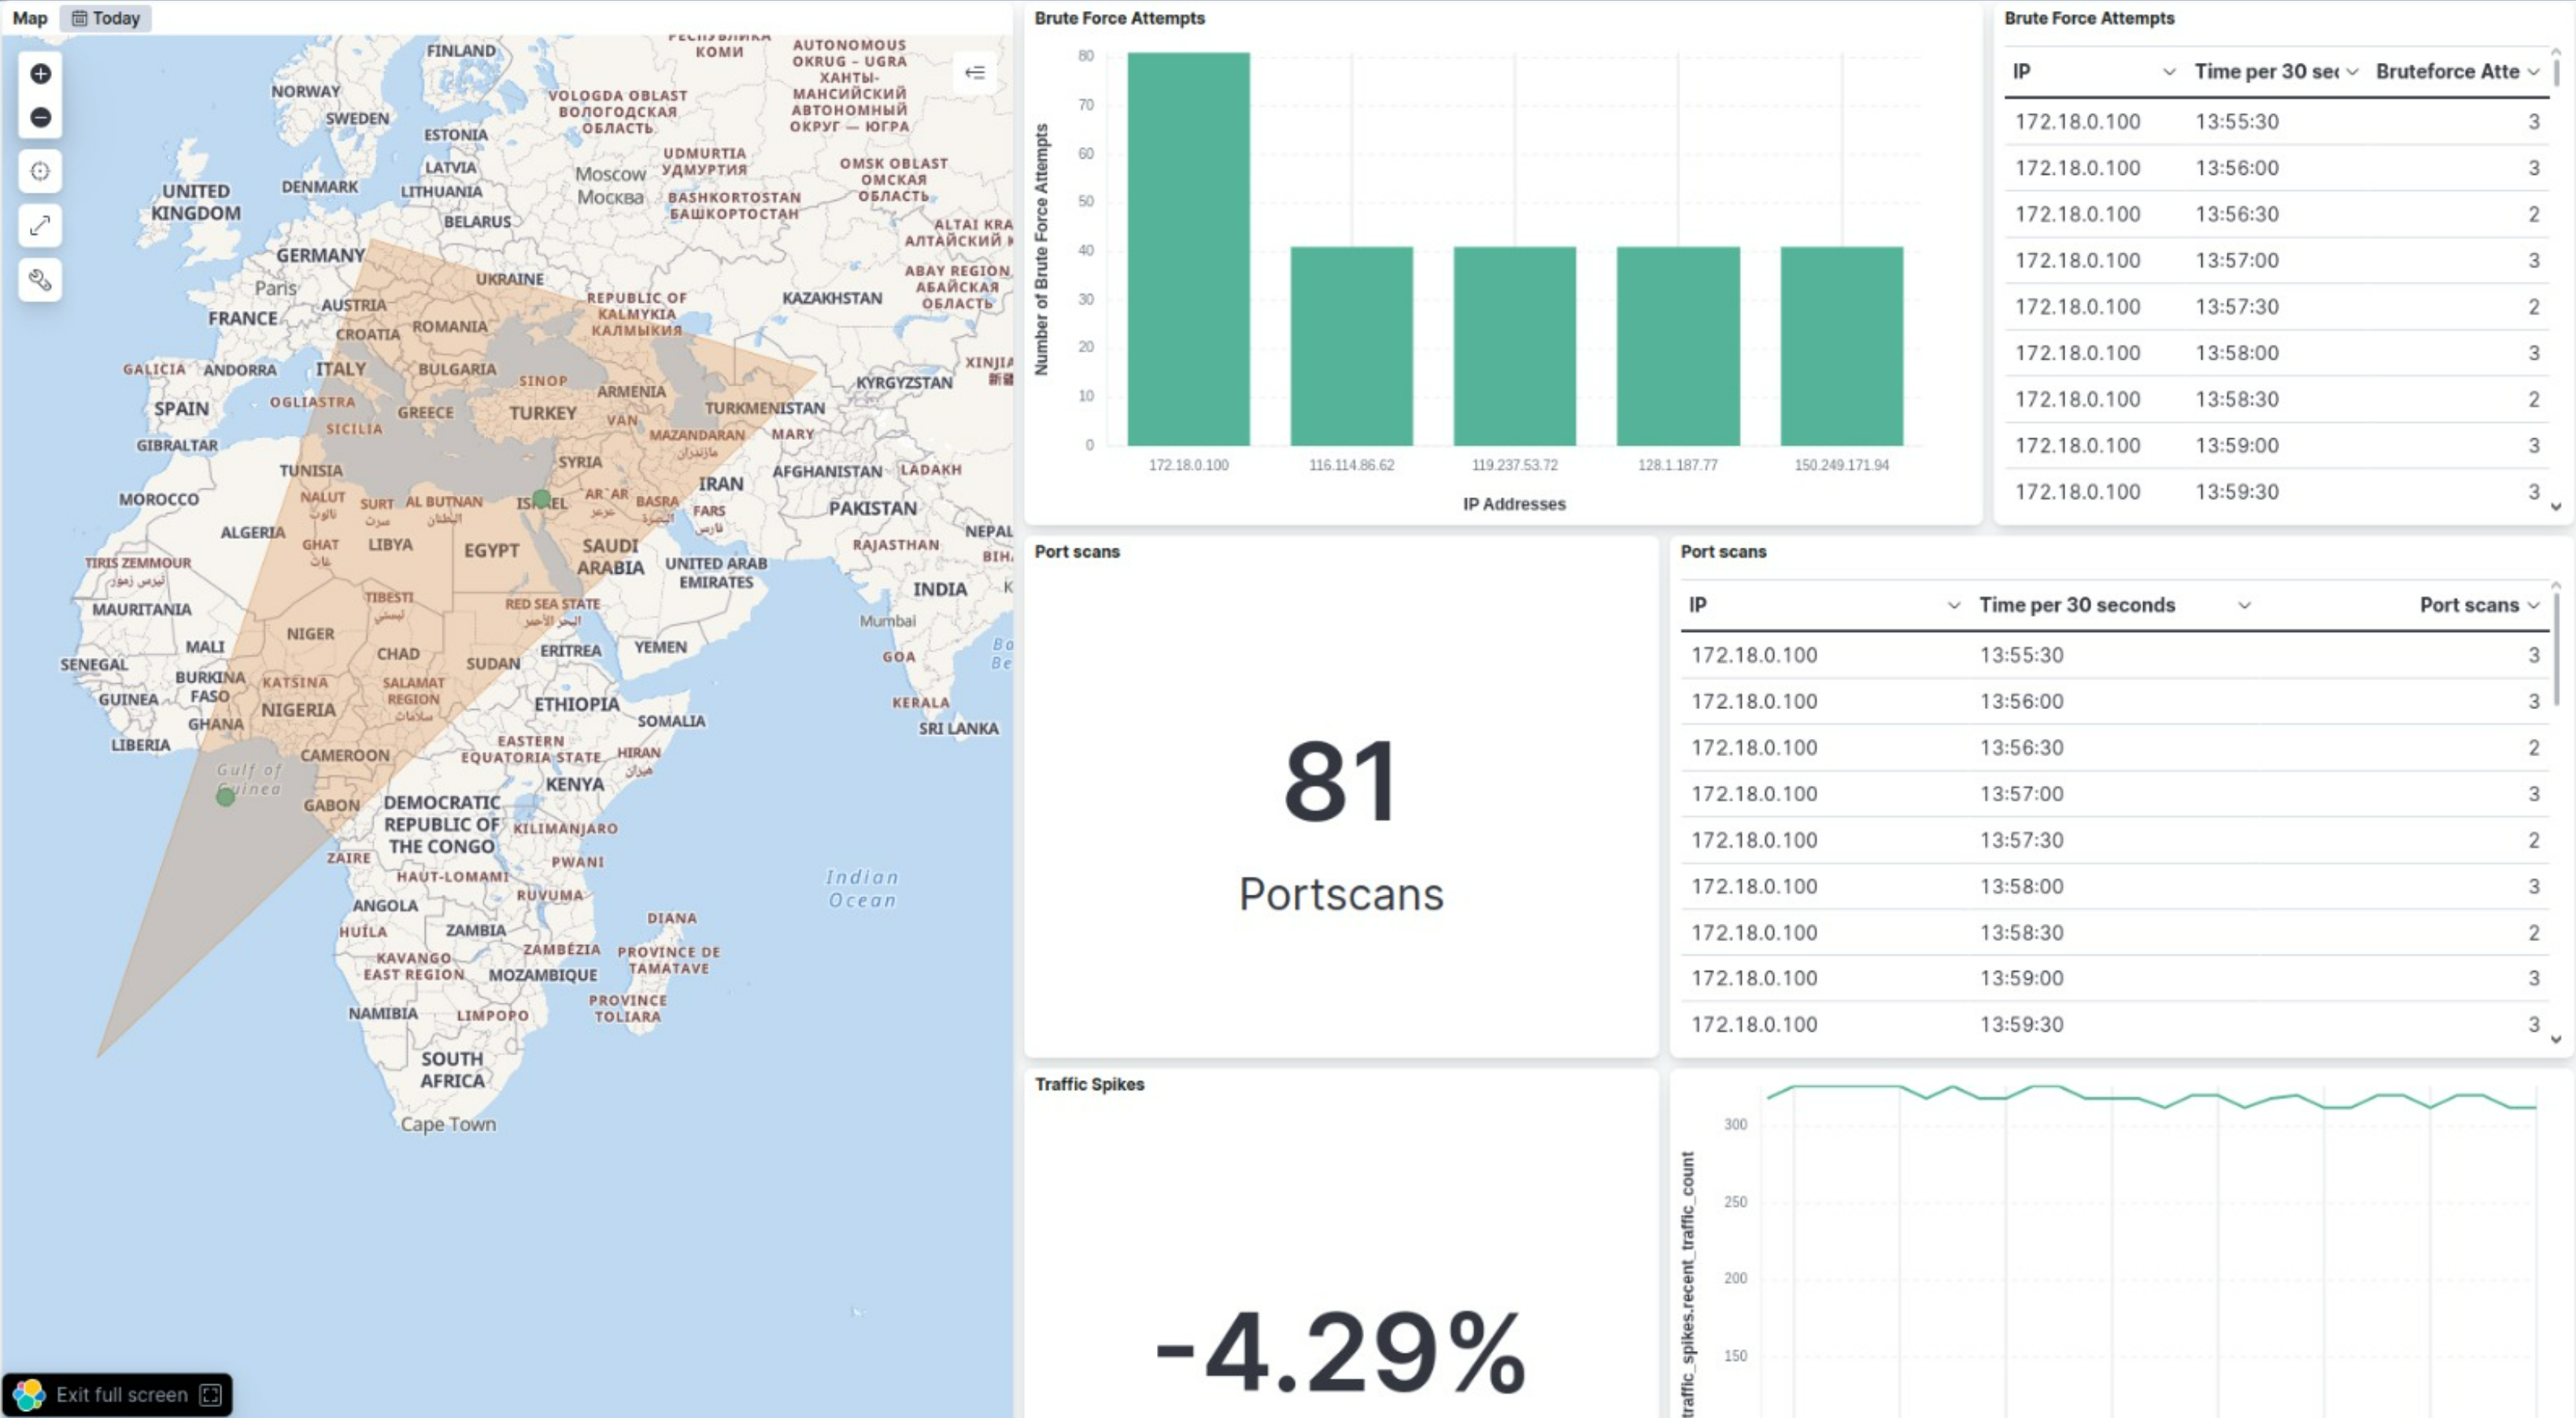
\includegraphics[width=\textwidth]{./images/dashboard.png}
        \caption{Dashboard in Kinbana}\label{fig:dashboard}
    \end{figure}

    \newpage
    \subsection{Discussion (Review of Results)}\label{subsec:discussion-(review-of-results)}
    The outcomes of this project indicate a substantial improvement in security monitoring capabilities.
    Our key results include:

    \begin{itemize}
        \item \textbf{Successful Deployment:} The software was deployed on Ubuntu servers with minimal resource usage, demonstrating its efficiency and low overhead.
        The installation process was streamlined, making it accessible even to users with limited technical expertise.
        \item \textbf{Accurate Detection:} The tool's ability to accurately detect and report unauthorized IP addresses was validated through rigorous testing and real-world application.
        The system's algorithms were fine-tuned to minimize false positives, ensuring that administrators receive reliable alerts.
        \item \textbf{User Feedback:} Early adopters provided positive feedback, particularly noting the ease of installation and user-friendly interface.
        This feedback has been invaluable for making further refinements and enhancements.
        Users reported that the intuitive dashboard and clear reporting formats significantly reduced the time required to respond to potential threats.
    \end{itemize}

    \noindent Moreover, the project’s open-source license has encouraged contributions from a broader community, enhancing the tool's functionality and security.
    The collaborative nature of open-source development has proven to be a significant strength, resulting in a more robust and versatile product.
    Community contributions have led to the addition of new features, improved documentation, and the identification and fixing of potential vulnerabilities.
    The impact of this project extends beyond immediate security improvements.
    By automating the detection and reporting of malicious IP addresses, the software frees up valuable time for system administrators.
    This allows them to focus on proactive security measures, such as threat analysis and infrastructure improvements, rather than being bogged down by routine monitoring tasks.
    This shift from reactive to proactive security management is a crucial step in enhancing overall cybersecurity posture.

    \subsection{Bottom Line («Fazit»)}\label{sec:fazit}
    The implementation of the Malicious IP-Address Monitor has demonstrated a significant productivity increase for system administrators.
    Below is a detailed analysis of the estimated productivity increase:

    \begin{table}[H]
        \begin{flushleft}
            \begin{tabularx}{\textwidth}{|X|X|X|X|}
                \hline
                \textbf{Activity} & \textbf{Time Saved per Week (hours)} & \textbf{Time Saved per Year (hours)} & \textbf{Cost Saving per Year (\$)} \\ \hline
                Manual Monitoring & 5                                    & 260                                  & 13,000                             \\ \hline
                Reporting         & 2                                    & 104                                  & 5,200                              \\ \hline
                Total             & 7                                    & 364                                  & 18,200                             \\ \hline
            \end{tabularx}
            \caption{Productivity Increase Analysis}
            \label{tab:productivity-analysis}
        \end{flushleft}
    \end{table}
    \vspace*{-2mm}

    \noindent The table clearly illustrates the time and cost savings achieved through the use of the Malicious IP-Address Monitor.
    By automating the monitoring and reporting process, system administrators can save significant time, which translates to substantial cost savings over the course of a year.
    The reduction in manual monitoring not only cuts costs but also reduces the risk of human error, which can be critical in maintaining secure systems.
    Automated alerts ensure that threats are identified and addressed promptly, reducing potential downtime and preventing security breaches that could lead to more significant financial and reputational damage.

    \newpage
    \subsection{Future Work}\label{subsec:Futur Work}
    Future improvements and extensions of this project could include:

    \begin{itemize}
        \item \textbf{Expanding Compatibility:} Broadening the software's compatibility to include other operating systems such as Windows and macOS. This will allow a wider range of users to benefit from the security enhancements offered by the tool.
        \item \textbf{Machine Learning Integration:} Integrating machine learning algorithms to predict and prevent potential attacks, enhancing the tool's proactive capabilities.
        Machine learning can help in identifying patterns and anomalies that traditional methods might miss, providing an additional layer of security.
        \item \textbf{User Interface Enhancements:} Continuously improving the user interface based on user feedback to ensure an optimal user experience.
        A more intuitive interface can help users to quickly understand and utilize the tool's features, leading to more effective security management.
        \item \textbf{Mobile Application Development:} Developing a mobile application for real-time alerts and monitoring, providing administrators with greater flexibility and responsiveness.
        With a mobile app, administrators can receive notifications and take action from anywhere, ensuring continuous protection.
        \item \textbf{DMARC Implementation:} Implementing DMARC (Domain-based Message Authentication, Reporting, and Conformance) to further enhance email security by preventing email spoofing and phishing attacks.
        This addition would provide an extra layer of protection, ensuring that incoming emails are authenticated against specific criteria and reported if they fail authentication.
    \end{itemize}

    \noindent In conclusion, the Malicious IP-Address Monitor has proven to be an effective tool in enhancing cybersecurity measures.
    The continuous support and contributions from the community will ensure its growth and adaptation to future challenges, making it a valuable asset in the fight against cyber threats.



    \newpage
    \begin{thebibliography}{9}

        \bibitem{cobalt2024}
        Cobalt. (2024). "Top Cybersecurity Statistics for 2024." Retrieved from \url{https://www.cobalt.io/blog/cybersecurity-statistics-2024}

        \bibitem{techwire2022}
        Tech Wire Asia. (2022). "Unauthorized access the biggest cause of data breaches." Retrieved from \url{https://techwireasia.com/07/2022/unauthorized-access-the-biggest-cause-of-data-breaches/#:~:text=As%20such%2C%20in%202021%2C%20its,increase%20from%20the%20previous%20year.}

        \bibitem{coalition2024}
        Coalition. (2024). "Cyber Threat Index 2024." Retrieved from \url{https://info.coalitioninc.com/download-cyber-threat-index-2024-b.html}

        \bibitem{talos2024}
        Cisco Talos. (2024). "Large-scale brute-force activity targeting VPNs, SSH services with commonly used login credentials." Retrieved from \url{https://blog.talosintelligence.com}

        \bibitem{securityweek2024}
        SecurityWeek. (2024). "Cisco: Multiple VPN, SSH Services Targeted in Mass Brute-Force Attacks." Retrieved from \url{https://www.securityweek.com}

        \bibitem{cyberpress2024}
        CyberPress. (2024). "Surge in Brute-Force SSH Attacks Targets Linux Servers." Retrieved from \url{https://cyberpress.org}

        \bibitem{sucuri2024}
        Sucuri. (2024). "How to Prevent SSH Brute Force Login Attacks." Retrieved from \url{https://blog.sucuri.net}

    \end{thebibliography}


% Appendix
    \appendix


    \newpage
    \section{Appendix}\label{sec:appendix}

    \subsection{Facsimile of Project Description}\label{subsec:facsimile-of-project-description}
    \begin{quote}
        \textbf{Malicious IP-Address Monitor}\\
        \textbf{Description:} The goal of this project is to deliver a FLOSS-licensed, platform-independent, Internet-connection-monitoring daemon, called Malicious IP-Address Monitor, that remotely monitors a Linux (Ubuntu) Internet (Email \& Web) server for unauthorized “sysadmin” traffic (unauthorized in-bound port scans, as well as unauthorized log-in attempts via SSH, FTP[S], and IMAP[S]) and that publishes the (unauthorized) IP-addresses corresponding to such activity to a pillory (German: Schandpfahl; like AbuseIPDB), so as to complement - by integrating - the existing FLOSS-DMARC-Demon for the monitoring of unauthorized email traffic (phish, spam, etc.) originating from unauthorized IP-addresses too.

        \noindent The purpose of this project is to make the Internet a safer space by complementing technological endpoint security measures (e.g., IPtables) with a psychological endpoint security measure (loss of the bad guys' faces), and thus to discourage attacks on Internet-servers (shaming of bad guys) and by helping cyber law enforcement do their job.\\

        \noindent The code should be minimal, modular, and self-explaining.
        The project report should be concise (maximally informative, minimally long).
        It must contain this project description as a quotation.

        \textbf{Technologies:}
        \begin{itemize}
            \item AbuseIPDB (\url{https://www.abuseipdb.com})
            \item DMARC-Demon (policies, reports; \url{https://github.com/soracel/dmarcvisualizer})
            \item IPtables (policies, connection log files; \url{https://en.wikipedia.org/wiki/Iptables})
        \end{itemize}

        \textbf{Literature:}
        \begin{itemize}
            \item \url{https://doi.org/10.1145/1592451.159245}
            \item \url{https://doi.org/10.1016/B978-0-12-411597-2.00007-2}
            \item \url{https://doi.org/10.1145/3139294} (Web-browser technology)
        \end{itemize}

        \textbf{Law enforcement:}
        \begin{itemize}
            \item \url{https://www.suisse-epolice.ch/home}
            \item \url{https://www.ncsc.admin.ch/ncsc/de/home.html}
        \end{itemize}

        \textbf{Advisor:}
        Dr. Simon KRAMER (\url{https://www.simon-kramer.ch/Simon-Kramer.vcf})
    \end{quote}


    \newpage
    \subsection{Declaration of Authorship}\label{subsec:declaration-of-authorship}
    The undersigned hereby declare that the accompanying report titled \("\)Malicious IP-Address Monitor: Enhancing Internet Security,\("\) submitted to the Bern University of Applied Sciences, is our original work.
    Contributions made by any other person, published or unpublished, have been duly acknowledged, and no material other than that listed has been used.\\

    \noindent This work has not been submitted for any other degree or professional qualification and is not currently being considered for publication elsewhere.\\

    \noindent We acknowledge the use of AI-based tools to assist with the improvement of the English writing in this report.
    The use of such technology was strictly limited to language enhancement and did not contribute to the original research, analysis, or conceptual development of the project.

    \vspace{1cm}
    \noindent\rule{6cm}{0.4pt}\\
    Pelletier Max

    \vspace{1cm}
    \noindent\rule{6cm}{0.4pt}\\
    Pernjak Stefani

    \vspace{1cm}
    \noindent\rule{6cm}{0.4pt}\\
    Rezzonico Marco

    \vspace{1cm}
    \noindent Date: \today

\end{document}
